
\documentclass[11pt,a4paper,openany]{report}
\usepackage[T1]{fontenc}
\usepackage[utf8]{inputenc}
\usepackage{lmodern}
\usepackage{microtype}
\usepackage{amsmath,amssymb,amsthm,mathtools,bm}
\usepackage{booktabs,array,longtable,tabularx}
\usepackage{xcolor}
\usepackage[margin=22mm,headheight=23pt]{geometry}
\usepackage{enumitem}
\usepackage{fancyhdr}
\usepackage{fancyvrb}
\usepackage{graphicx}
\usepackage{url}
\usepackage{xurl}
\usepackage{hyperref}
\definecolor{finblue}{HTML}{1F5A99}
\definecolor{fingreen}{HTML}{19733A}
\definecolor{finorange}{HTML}{D55E00}
\definecolor{finred}{HTML}{A61B1B}
\definecolor{finviolet}{HTML}{6A3D9A}
\definecolor{fingray}{HTML}{4D4D4D}

\hypersetup{
  unicode=true,colorlinks=true,linkcolor=finblue,citecolor=fingreen,
  urlcolor=finblue,
  pdftitle={Second-Generation Atlas: Derived Nadsoliton Objects},
  pdfauthor={Krzysztof Żuchowski},
  pdfsubject={Systematic search over FIN combinations C01--C12, objects O01--O15, and synthesis G01--G10},
  pdfkeywords={FIN, nadsoliton, Stieltjes functions, Schur complement, memory kernel, operator theory, information geometry}
}
\pagestyle{fancy}
\fancyhf{}
\fancyhead[L]{\small Second-Generation Atlas}
\fancyhead[R]{\small Release 10.23 --- English edition}
\fancyfoot[C]{\thepage}

\setlength{\parindent}{0pt}
\setlength{\parskip}{0.55em}
\setlist{nosep,leftmargin=2em}
\setcounter{tocdepth}{2}
\setcounter{secnumdepth}{3}
\emergencystretch=3em
\newcommand{\one}{\bm 1}
\newcommand{\C}{\mathbb C}
\newcommand{\R}{\mathbb R}
\newcommand{\Z}{\mathbb Z}
\newcommand{\statusProven}{\textcolor{fingreen}{[Proven]}}
\newcommand{\statusStrong}{\textcolor{finblue}{[Strong evidence]}}
\newcommand{\statusModerate}{\textcolor{finviolet}{[Moderate evidence]}}
\newcommand{\statusWeak}{\textcolor{fingray}{[Weak evidence]}}
\newcommand{\statusSpeculative}{\textcolor{finorange}{[Speculative]}}
\newcommand{\statusRefuted}{\textcolor{finred}{[Refuted]}}

\begin{document}
\hypersetup{pageanchor=false}
\begin{titlepage}
\centering
\vspace*{12mm}
{\Large\bfseries FIN --- Release 10.23\par}
\vspace{12mm}
{\Huge\bfseries Second-Generation Atlas\par}
\vspace{5mm}
{\LARGE\bfseries Derived Nadsoliton Objects\par}
\vspace{8mm}
{\Large Systematic search over C01...C12,\\
construction of O01...O15, and synthesis of G01...G10\par}
\vspace{18mm}
{\Large Krzysztof \.Zuchowski\par}
\vspace{2mm}
{\normalsize Independent Researcher --- Fractal Information Theory Project\par}
\vspace{2mm}
{\normalsize ORCID: \href{https://orcid.org/0009-0002-0909-3613}{0009-0002-0909-3613}\par}
\vspace{10mm}
{\large 28 July 2026\par}
\vfill
\begin{minipage}{0.9\textwidth}
\small
\textbf{Central object.}
\[
E\longmapsto \operatorname{Schur}_{V\setminus E}(zI+A),\qquad
\Sigma_E(z)=A_{EH}(zI+A_{HH})^{-1}A_{HE}.
\]
Contextual reductions compose, while self-energies are positive
operator-valued Stieltjes functions generating exact memory.

\medskip
\textbf{Boundary.} This report does not export a selector, physical scale,
legacy--strict bridge, role transfer, or laboratory validation.

\medskip
\textbf{Repository.}
\url{https://github.com/hyconiek/Fractal-Nadsoliton-Theory}

\textbf{License.} CC BY 4.0.
\end{minipage}
\vfill
\end{titlepage}
\hypersetup{pageanchor=true}
\pagenumbering{roman}
\tableofcontents
\clearpage
\pagenumbering{arabic}

\chapter*{Confidence convention}
\addcontentsline{toc}{chapter}{Confidence convention}

\begin{itemize}
\item 
\textbf{\statusProven{}} --- an analytic result or an explicit numerical identity within a stated tolerance.

\item 
\textbf{\statusStrong{}} --- a stable construction whose general theorem or interpretation remains open.

\item 
\textbf{\statusModerate{}} --- a typed mechanism whose identifiability or uniqueness remains open.

\item 
\textbf{\statusSpeculative{}} --- a constructive hypothesis intended for falsification.

\item 
\textbf{\statusRefuted{}} --- a connection rejected in the stated class, usually because no common typed operation exists.

\end{itemize}

\chapter{Executive summary}

The second phase of the atlas no longer asks only what the puzzles C01...C12 resemble. It asks:

\[
\text{which new objects can be constructed by composing their operations?}
\]

A finite, reproducible search was performed:

\begin{center}
\begingroup\small
\setlength{\tabcolsep}{2.5pt}
\renewcommand{\arraystretch}{1.16}
\begin{longtable}{@{}p{0.420\textwidth}p{0.420\textwidth}@{}}
\toprule
\textbf{Class} & \textbf{Count} \\
\midrule
\endhead
individual puzzles & 12 \\
all pairs & 66 \\
all triples & 220 \\
selected couplings of 4--6 puzzles & 7 \\
combinations scanned in total & 305 \\
rows yielding a typed object or mechanism & 109 \\
purely visual combinations rejected & 184 \\
second-generation O-objects & 15 \\
third-generation G-objects & 10 \\
\bottomrule
\end{longtable}
\endgroup
\end{center}

\begin{figure}[htbp]
\centering
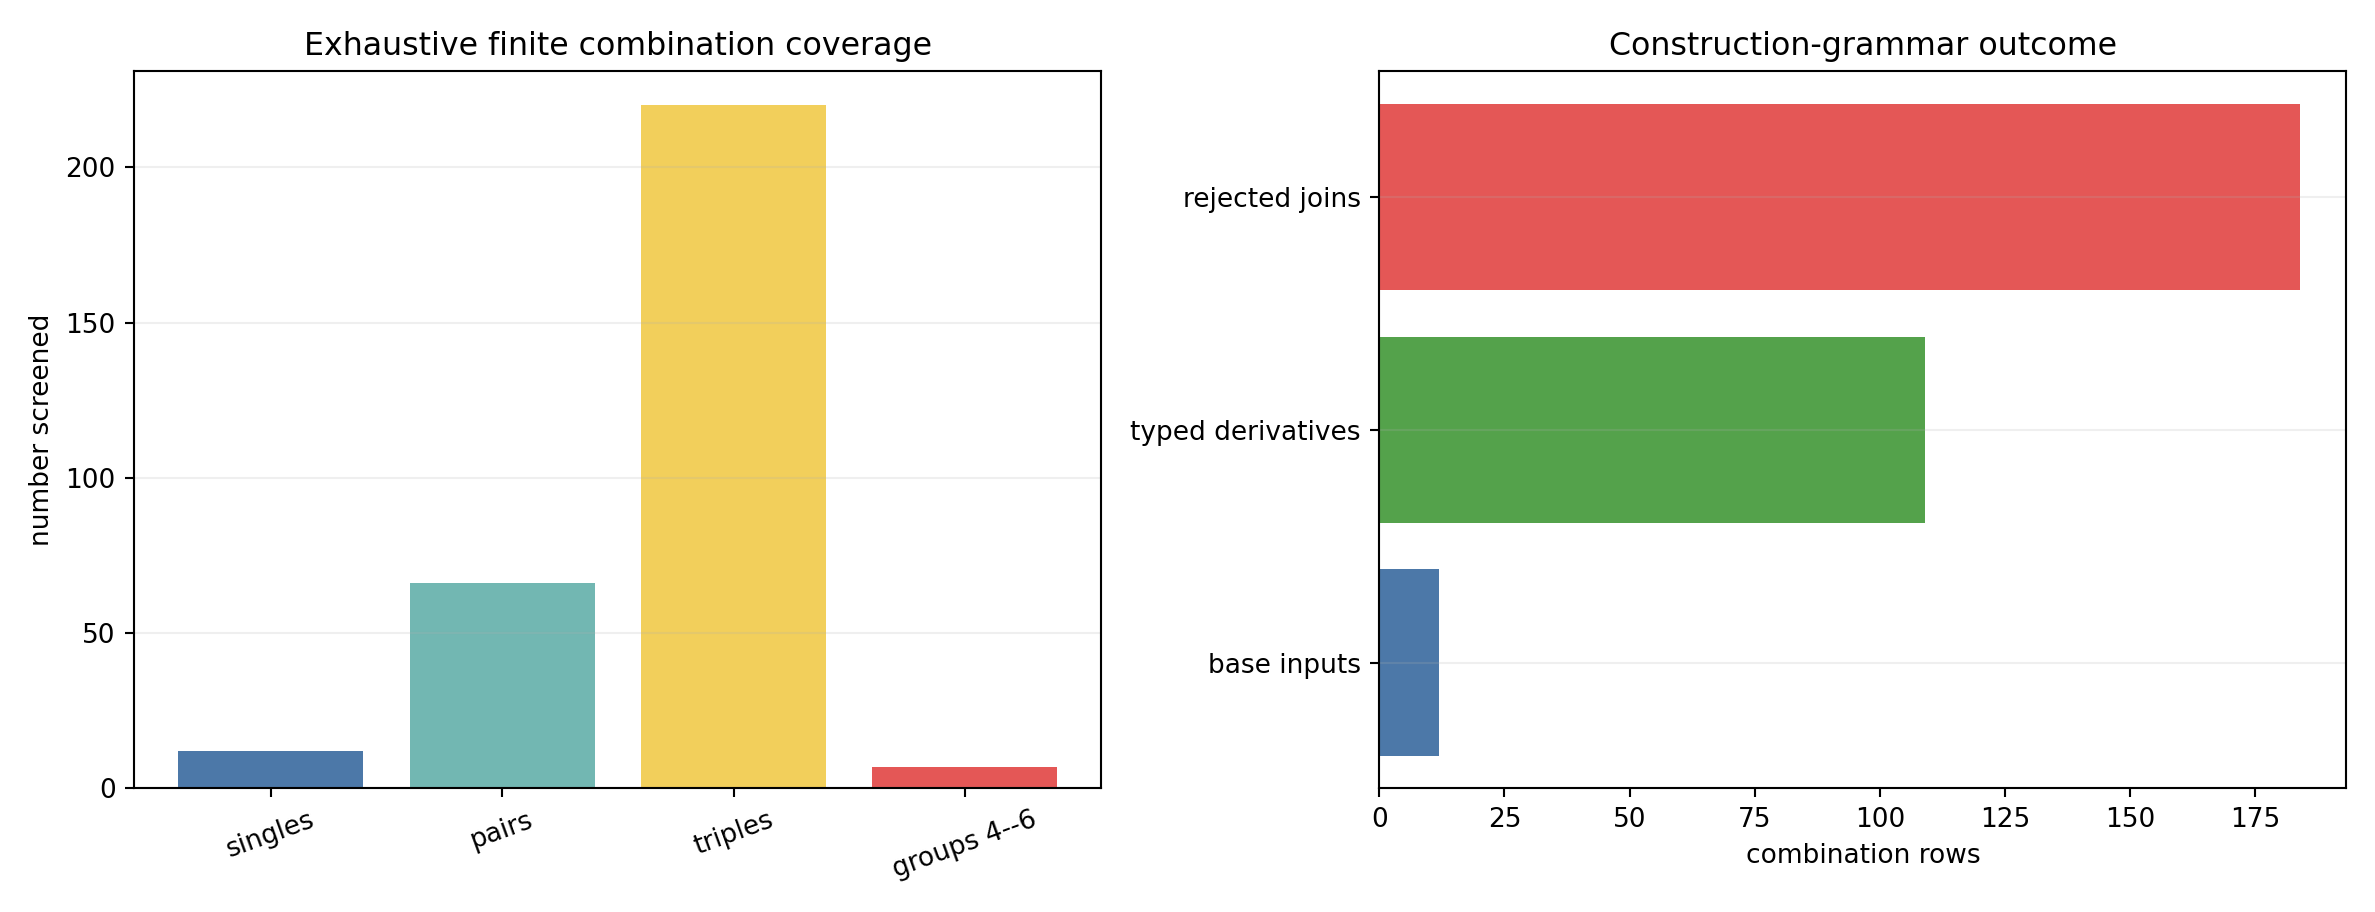
\includegraphics[width=0.97\textwidth]{FIN_Second_Generation_Atlas_Figures/combination_search_coverage.png}
\caption{Complete coverage of singles, pairs, and triples, together with the output of the explicit construction grammar.}
\end{figure}

The strongest derived object is not a single matrix but a contextual family:

\[
\mathfrak S_A:
E\longmapsto
B_E(z)
=\operatorname{Schur}_{V\setminus E}(zI+A),
\qquad z>0.
\]

For every observed context \(E\), the hidden sector generates the self-energy

\[
\Sigma_E(z)
=A_{EH}(zI+A_{HH})^{-1}A_{HE}.
\]

This family has three exact properties:

\begin{enumerate}
\item 
nested reductions compose exactly by associativity of the Schur complement;

\item 
\(\Sigma_E(z)\) is a positive operator-valued Stieltjes function;

\item 
its inverse Laplace transform is the memory kernel of the reduced process.

\end{enumerate}

We call the resulting G02 object the \textbf{Stieltjes--Schur Context Functor}.

It is \textbf{\statusProven{}} as finite operator algebra and \textbf{\statusSpeculative{}} as a foundation for physical ontology.

The second particularly promising object is the chiral memory susceptibility

\[
\Xi_E(z)
=
\left.
\partial_\theta\Sigma_E(z,\theta)
\right|_{\theta=0}.
\]

It is nonzero and odd under reflection, but it is a \textbf{receiver} of the inserted twist \(\theta\), not a source of orientation. \textbf{\statusStrong{}}

The third result clarifies "negative information coupling." Loss of accessible information can be represented without modifying the kernel by the contraction ledger

\[
\mathcal L_t(p,q)
=D(p\Vert q)-D(P_tp\Vert P_tq)\geq0.
\]

This is loss of distinguishability in the accessible channel. It is not automatically destruction of information or thermodynamic energy. \textbf{\statusProven{}}

\chapter{Generation rather than analogy matching}

Every combination passes through five gates:

\begin{enumerate}
\item 
\textbf{Common operation:} can the puzzle operations be composed with compatible input and output types?

\item 
\textbf{New object:} is the output more than a list of constituents?

\item 
\textbf{New space:} does the object live in a recognizable space of operators, functionals, measures, or functors?

\item 
\textbf{Observable and dynamics:} does the construction provide a testable number, record, or evolution?

\item 
\textbf{Falsification gate:} what outcome would refute the construction or its stronger interpretation?

\end{enumerate}

Stop rule:

\begin{quote}\itshape
A combination without a typed operation does not generate an object. Verbal or visual resemblance alone is marked \statusRefuted{}.

\end{quote}

The complete result for all 305 combinations is stored in FIN\_Second\_Generation\_Combination\_Search.csv. Each row records the common operation, candidate object, object space, new observable, new dynamics, status, and whether the result is a new coupling or merely inherits a lower-order object.

\chapter{Base inventory C01...C12}

\begin{center}
\begingroup\small
\setlength{\tabcolsep}{2.5pt}
\renewcommand{\arraystretch}{1.16}
\begin{longtable}{@{}p{0.055\textwidth}p{0.200\textwidth}p{0.420\textwidth}p{0.185\textwidth}@{}}
\toprule
\textbf{ID} & \textbf{Base object} & \textbf{Dominant operation} & \textbf{Critical limitation} \\
\midrule
\endhead
C01 & strict kernel & convolution/\allowbreak{}spectralization on \(Z_{12}\) & no automatic continuum \\
C02 & legacy intermediate bridge & propagator-like damped profile & no complete completion map or role transfer \\
C03 & \(A=sI-W\succeq0\) & Dirichlet form and spectral calculus & no energy unit \\
C04 & \(e^{-itA},e^{-tA}\) & two rays of functional calculus & different operational semantics \\
C05 & Green/\allowbreak{}resolvent/\allowbreak{}action & operator inversion and variation & propagator does not determine the full interaction \\
C06 & cocycle/\allowbreak{}chiral receivers & sign under inversion & no non-premise sign \\
C07 & fractal Schur compression & elimination of degrees of freedom & strict is not a static fixed point \\
C08 & adaptation and memory & operator--record feedback & learning law is additional input \\
C09 & information/\allowbreak{}geometry & entropy, Fisher metric, diffusion & no physical unit \\
C10 & operational process & preparation--instrument--environment--record & concrete laboratory remains external \\
C11 & scale obstruction & quotient by \(\mathbb R_{>0}\) & no canonical section \\
C12 & selector obstruction & orientation quotient/\allowbreak{}torsor & QW-2191 remains open \\
\bottomrule
\end{longtable}
\endgroup
\end{center}

\chapter{Main table: second-generation objects}

\begin{center}
\begingroup\fontsize{7}{8.4}\selectfont
\setlength{\tabcolsep}{2.5pt}
\renewcommand{\arraystretch}{1.16}
\begin{longtable}{@{}p{0.083\textwidth}p{0.157\textwidth}p{0.267\textwidth}p{0.139\textwidth}p{0.159\textwidth}p{0.055\textwidth}@{}}
\toprule
\textbf{FIN combination} & \textbf{Derived object} & \textbf{Mathematical form} & \textbf{Analogous fields} & \textbf{New intuition} & \textbf{Status} \\
\midrule
\endhead
C03+\allowbreak{}C05+\allowbreak{}C07 & O01 Dynamic Spectral Compression Kernel & \(\Sigma_E(z)=A_{EH}(zI+A_{HH})^{-1}A_{HE}\) & Feshbach, Mori--Zwanzig, Kron reduction & dynamic reduction generates memory & \statusProven{} \\
C03+\allowbreak{}C05+\allowbreak{}C07 & O02 Frequency-Dependent Effective Action & \(S_z[x]=\frac12\langle x,(zI+A_{EE}-\Sigma_E(z))x\rangle-\langle j,x\rangle\) & effective action, influence functional & Green, compression, and variation become one object & \statusProven{} \\
C05+\allowbreak{}C07+\allowbreak{}C10 & O03 Resolvent Context Presheaf & \(E\mapsto\operatorname{Schur}_{V\setminus E}(zI+A)\) & category theory, open systems, network reduction & each observer/\allowbreak{}context has a compatible effective operator & \statusProven{} \\
C03+\allowbreak{}C06+\allowbreak{}C12 & O04 Chiral Spectral Response Bundle & \((M_R,\Lambda,C_\chi,\operatorname{Im}B)\) & asymmetry resources, harmonic analysis & distinct sign receivers detect one resource type & \statusStrong{} \\
C06+\allowbreak{}C07+\allowbreak{}C10 & O05 Chiral Memory Susceptibility & \(\Xi_E(z)=\partial_\theta\Sigma_E(z,\theta)|_0\) & Kubo response, flux susceptibility, open systems & hidden degrees of freedom possess chiral memory response & \statusStrong{} \\
C03+\allowbreak{}C04+\allowbreak{}C09 & O06 Heat Information Metric Tower & \(D_t^2(x,y)=\sum_z|P_t(x,z)-P_t(y,z)|^2/\pi_z\) & diffusion maps, information geometry & informational distance is multiscale & \statusProven{} \\
C10+\allowbreak{}C11 & O07 Operational Calibration Torsor & \((A,\tau)\sim(cA,\tau/c)\) & metrology, gauge fixing, identification & experiment selects scale; algebra supplies an orbit & \statusProven{} \\
C01+\allowbreak{}C03+\allowbreak{}C11 & O08 Projective Spectral Fingerprint & \((\lambda_1/\lambda_{\max},\ldots)\) & inverse spectral theory, control & part of the prediction is testable before absolute calibration & \statusProven{} \\
C04+\allowbreak{}C09+\allowbreak{}C10 & O09 Information Contraction Ledger & \(\mathcal L_t=D(p\Vert q)-D(P_tp\Vert P_tq)\) & data processing, statistics, sensory bottlenecks & "loss" is loss of accessible distinguishability & \statusProven{} \\
C04+\allowbreak{}C07+\allowbreak{}C10 & O10 Dual-Ray Reduced Process Tensor & \(\mathcal T_r[\mathcal M_1,\ldots,\mathcal M_r]\) for wave/\allowbreak{}heat projections & process tensors, cybernetics, causal models & memory becomes visible through multitime interventions & \statusModerate{} \\
C08+\allowbreak{}C09+\allowbreak{}C10 & O11 Adaptive Memory Geometry Flow & \((\dot A,\dot q)=(-\nabla_A\mathcal L,-\operatorname{grad}_F\mathcal L)\) & neural operators, adaptive networks, plasticity & learning may occur in memory-geometry space & \statusSpeculative{} \\
C05+\allowbreak{}C07+\allowbreak{}C08 & O12 Multiscale Memory Functor & \(\Sigma^{(0)}(z)\to\Sigma^{(1)}(z)\to\cdots\) & continued fractions, hierarchical reservoirs, RG & seek a fractal fixed point in memory-function space & \statusStrong{} \\
C01+\allowbreak{}C02+\allowbreak{}C07 & O13 Legacy-Strict Completion-Defect Tower & \(\Delta_n=K_{\rm strict}^{(n)}-\mathcal C_n[K_{\rm legacy}^{(n)}]\) & error propagation, RG defects, obstruction theory & study bridge failure dynamically instead of asserting similarity & \statusModerate{} \\
C06+\allowbreak{}C09+\allowbreak{}C12 & O14 Spectral Asymmetry Transport Cost & \(\inf_{\Phi\ {\rm covariant}}\operatorname{Cost}(\Phi)\) & optimal transport, resource conversion & orientation has operational cost, but cost does not select a sign & \statusModerate{} \\
C10+\allowbreak{}C11+\allowbreak{}C12 & O15 Two-Torsor Physicalization Bundle & \(\mathcal T_{\rm scale}\times\mathcal T_{\rm orient}\) & principal bundles, frames, calibration & scale and orientation require separate sections & \statusStrong{} \\
\bottomrule
\end{longtable}
\endgroup
\end{center}

\chapter{Explanatory power and falsification}

\begin{center}
\begingroup\small
\setlength{\tabcolsep}{2.5pt}
\renewcommand{\arraystretch}{1.16}
\begin{longtable}{@{}p{0.140\textwidth}p{0.254\textwidth}p{0.197\textwidth}p{0.270\textwidth}@{}}
\toprule
\textbf{Derived object} & \textbf{What it explains} & \textbf{What it does NOT explain} & \textbf{Falsifying test} \\
\midrule
\endhead
O01 DSCK & exact memory after elimination & physical environment and scale & constant \(\Sigma_E(z)\) despite nonzero coupling \\
O02 Effective Action & exact contextual source response & nonlinear interactions and quantization & stationary solution disagrees with block Green function \\
O03 Context Presheaf & compatibility of nested reductions & unique observer context & nonzero direct-versus-nested residual \\
O04 Chiral Bundle & common covariance of sign receivers & source of sign & symmetric state with a nonzero odd receiver \\
O05 Chiral Memory & memory response to phase twist & selector for \(\theta\) & loss of oddness under reflection \\
O06 Metric Tower & geometry of distinguishability & SI length or Lorentz signature & distance grows under a contractive semigroup \\
O07 Calibration Torsor & non-identifiability of absolute scale & laboratory reference source & distinguish \((A,\tau)\) from \((cA,\tau/c)\) using the same \(P_\tau\) \\
O08 Fingerprint & scale-free spectral predictions & absolute energy & fingerprint changes under positive rescaling \\
O09 Information Ledger & accessible loss of distinguishability & thermodynamic energy or ontological destruction & violation of data processing \\
O10 Process Tensor & operational memory and interventions & concrete microscopic dilation & a memoryless model reproduces all interventions \\
O11 Adaptive Flow & possible operator-learning mechanism & strict source law or biology & no hold-out advantage over a static model \\
O12 Memory Functor & hierarchical dynamic compression & a strict fixed point & no stabilization of any functional class \\
O13 Defect Tower & where the bridge fails & role transfer and completion theorem & residual converges to zero without target coding \\
O14 Transport Cost & amount of asymmetry resource required & canonical choice of that resource & free operation increases the monotone \\
O15 Two-Torsor Bundle & independence of scale and orientation problems & source of either section & one internal datum canonically closes both torsors \\
\bottomrule
\end{longtable}
\endgroup
\end{center}

\chapter{Ranking O01...O15}

Scores use novelty, mathematical rigor, FIN relevance, and falsifiability from 0 to 5. Overinterpretation risk also ranges from 0 to 5, where 5 is highest.

\begin{figure}[htbp]
\centering
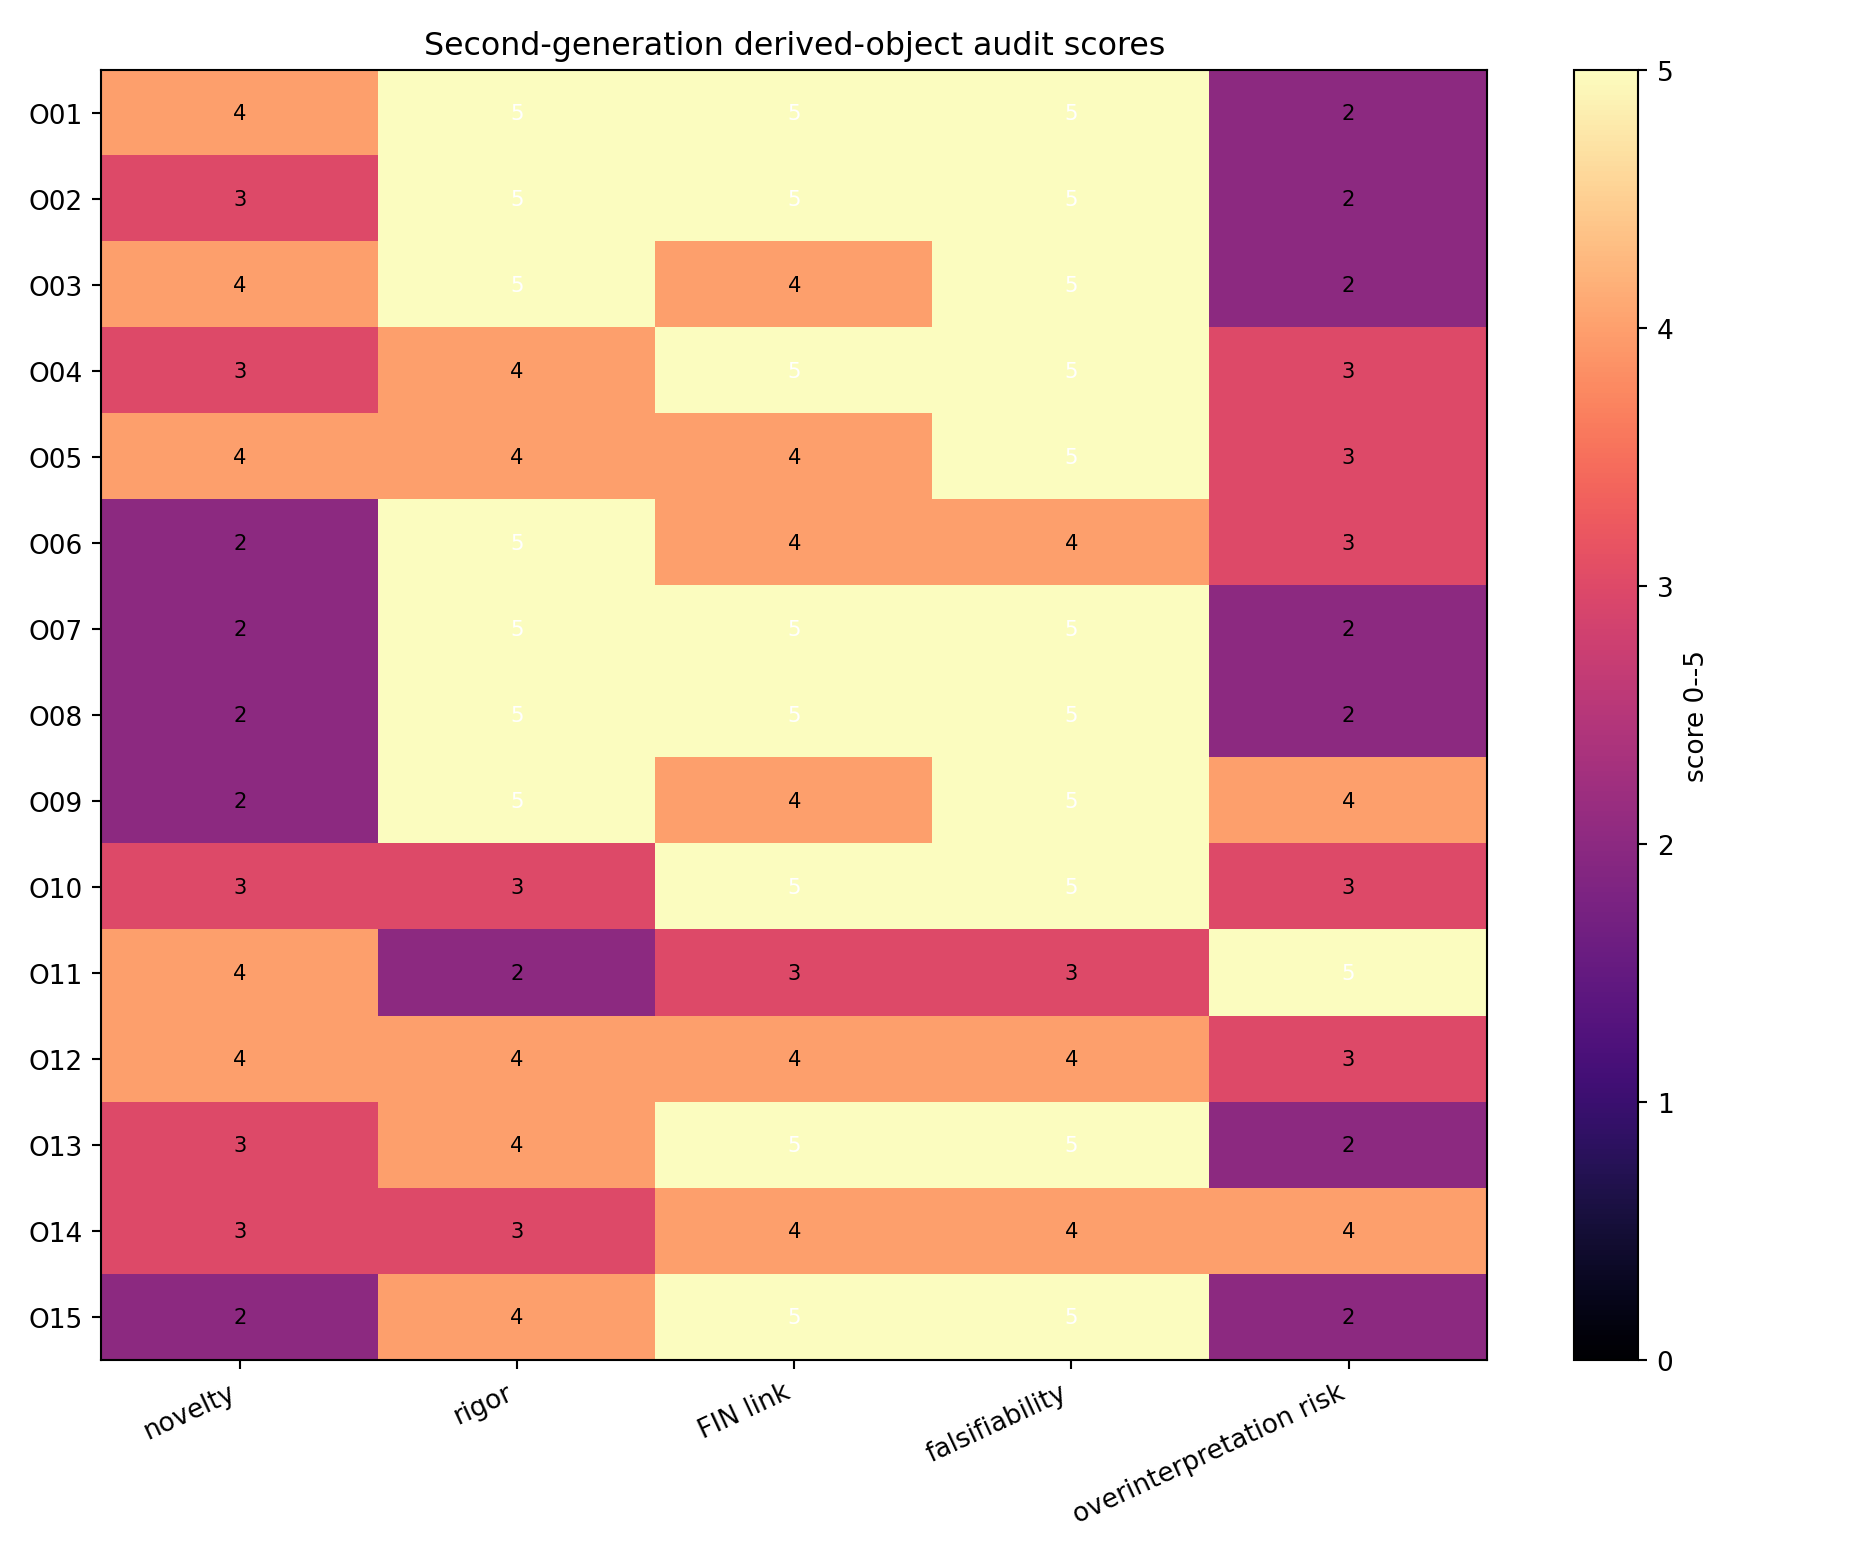
\includegraphics[width=0.97\textwidth]{FIN_Second_Generation_Atlas_Figures/derived_object_score_matrix.png}
\caption{Audit scores for O01--O15. Overinterpretation risk has the opposite semantics from the other scores.}
\end{figure}

\begin{center}
\begingroup\fontsize{7}{8.4}\selectfont
\setlength{\tabcolsep}{2.5pt}
\renewcommand{\arraystretch}{1.16}
\begin{longtable}{@{}p{0.072\textwidth}p{0.167\textwidth}p{0.119\textwidth}p{0.072\textwidth}p{0.334\textwidth}p{0.096\textwidth}@{}}
\toprule
\textbf{ID} & \textbf{Novelty} & \textbf{Rigor} & \textbf{FIN} & \textbf{Falsifiability} & \textbf{Risk} \\
\midrule
\endhead
O01 & 4 & 5 & 5 & 5 & 2 \\
O02 & 3 & 5 & 5 & 5 & 2 \\
O03 & 4 & 5 & 4 & 5 & 2 \\
O04 & 3 & 4 & 5 & 5 & 3 \\
O05 & 4 & 4 & 4 & 5 & 3 \\
O06 & 2 & 5 & 4 & 4 & 3 \\
O07 & 2 & 5 & 5 & 5 & 2 \\
O08 & 2 & 5 & 5 & 5 & 2 \\
O09 & 2 & 5 & 4 & 5 & 4 \\
O10 & 3 & 3 & 5 & 5 & 3 \\
O11 & 4 & 2 & 3 & 3 & 5 \\
O12 & 4 & 4 & 4 & 4 & 3 \\
O13 & 3 & 4 & 5 & 5 & 2 \\
O14 & 3 & 3 & 4 & 4 & 4 \\
O15 & 2 & 4 & 5 & 5 & 2 \\
\bottomrule
\end{longtable}
\endgroup
\end{center}

O01 has the best balance. O01+O03+O12 yields the richest higher-order structure. O11 has the greatest overinterpretation risk because analogies with learning and biology are not FIN source laws.

\chapter{Theorems generated in the second phase}

\section{O01 belongs to the operator Stieltjes class}

For \(z>0\) and \(A_{HH}\succeq0\),

\[
\Sigma_E(z)=A_{EH}(zI+A_{HH})^{-1}A_{HE}.
\]

For every \(n\geq0\),

\[
(-1)^n\Sigma_E^{(n)}(z)
=n!A_{EH}(zI+A_{HH})^{-(n+1)}A_{HE}\succeq0.
\]

Thus \(\Sigma_E\) is a completely monotone positive operator-valued function. \textbf{\statusProven{}}

Its poles and spectral measure encode hidden modes; its inverse Laplace transform is a decaying memory kernel. Consequently, the admissible space for dynamic compression is far narrower than the set of all matrix-valued functions. For strict \(Z_{12}\), orders \(0,\ldots,4\) have minimum eigenvalues above \(-6.4\times10^{-17}\), consistent with positivity up to floating-point error.

\section{O03 composes functorially}

Let \(G\subset F\subset E\subset V\). For \(B(z)=zI+A\),

\[
\operatorname{Schur}_{E\setminus G}
\left(\operatorname{Schur}_{V\setminus E}B\right)
=\operatorname{Schur}_{V\setminus G}B.
\]

This is associativity of Gaussian elimination/\allowbreak{}the Schur complement. \textbf{\statusProven{}} The direct-versus-nested residual in selected strict \(Z_{12}\) contexts is \(2.47\times10^{-16}\).

"Functor" is used in the restricted sense that the context poset and reduction morphisms form a compatible operator diagram. No sheaf axioms or quantum contextuality theorem are claimed.

\section{O02 reconstructs the exact contextual Green function}

Set

\[
B_E(z)=zI+A_{EE}-\Sigma_E(z).
\]

The functional

\[
S_z[x;j]=\frac12\langle x,B_E(z)x\rangle-\langle j,x\rangle
\]

has stationary solution

\[
x_\star=B_E(z)^{-1}j
=\left[(zI+A)^{-1}\right]_{EE}j.
\]

The audited stationarity residual is \(4.90\times10^{-16}\). \textbf{\statusProven{}} This exactly reconstructs an effective action from the resolvent. It is not a complete physical action because \(z\), the action unit, measure, and interactions remain additional data.

\section{O05: memory has a chiral response direction}

Introduce a Hermitian twisted family \(A(\theta)\), in which a hop by \(d\) acquires phase \(e^{id\theta}\). Then

\[
\Xi_E(z)=
\left.\partial_\theta
\left[
A_{EH}(\theta)(zI+A_{HH}(\theta))^{-1}A_{HE}(\theta)
\right]\right|_{\theta=0}.
\]

For the even/\allowbreak{}odd split of strict \(Z_{12}\),

\[
\|\Xi_E(0.2)\|_2=1.2175076427.
\]

For reflection \(R\),

\[
R_E\Xi_E(z)R_E=-\Xi_E(z),
\]

with residual \(2.17\times10^{-16}\). \textbf{\statusProven{}} for the stated twisted family and split.

Likewise,

\[
C_\chi=
\left.\frac{d}{d\theta}\operatorname{Tr}[\rho A(\theta)]
\right|_{\theta=0}
\]

has residual \(3.23\times10^{-13}\), promoting \(C_\chi\) from an ad hoc indicator to an explicit flux-twist response. The twist and its sign are still inserted in the test family; O05 does not discharge QW-2191.

\section{O09: negative informational coupling as channel contraction}

For a Markov channel \(P_t\) and positive distributions \(p,q\),

\[
D(P_tp\Vert P_tq)\leq D(p\Vert q).
\]

Define

\[
\mathcal L_t(p,q)=D(p\Vert q)-D(P_tp\Vert P_tq)\geq0.
\]

Across 1000 deterministically reproducible pairs:

\begin{center}
\begingroup\small
\setlength{\tabcolsep}{2.5pt}
\renewcommand{\arraystretch}{1.16}
\begin{longtable}{@{}p{0.420\textwidth}p{0.420\textwidth}@{}}
\toprule
\textbf{Quantity} & \textbf{Result} \\
\midrule
\endhead
minimum \(\mathcal L_t\) & 0.0485457 \\
median & 0.718427 \\
maximum & 3.15526 \\
violations below \(-10^{-12}\) & 0 \\
\bottomrule
\end{longtable}
\endgroup
\end{center}

This is \textbf{\statusProven{}} as an instance of the data-processing theorem. It is methodologically preferable to inserting "negative information" into a scalar kernel because it identifies the two hypotheses, the contracting channel, and the difference between inaccessible and destroyed information. It does not pretend to be energy without temperature and scale.

\section{O07+O08: exact calibration orbit}

\[
e^{-\tau A}=e^{-(\tau/c)(cA)}.
\]

The residual at \(c=7.25\) is \(3.43\times10^{-17}\), and the spectral fingerprint remains invariant with residual \(6.66\times10^{-16}\). \textbf{\statusProven{}}

An experiment can therefore test a scale-free fingerprint first, but physical time requires an external calibration section.

\section{O06: heat geometry contracts}

The maximum squared diffusion distance on \(Z_{12}\) is:

\begin{center}
\begingroup\small
\setlength{\tabcolsep}{2.5pt}
\renewcommand{\arraystretch}{1.16}
\begin{longtable}{@{}p{0.420\textwidth}p{0.420\textwidth}@{}}
\toprule
\textbf{\(t\)} & \textbf{\(\max_{x,y}D_t^2(x,y)\)} \\
\midrule
\endhead
0.10 & 17.3358 \\
0.25 & 11.0222 \\
0.50 & 5.69186 \\
1.00 & 2.00931 \\
\bottomrule
\end{longtable}
\endgroup
\end{center}

\textbf{\statusProven{}} for the tested family. The information geometry exists, but it is dimensionless and semigroup-time dependent.

\chapter{Second-order analogies}

\begin{center}
\begingroup\fontsize{7}{8.4}\selectfont
\setlength{\tabcolsep}{2.5pt}
\renewcommand{\arraystretch}{1.16}
\begin{longtable}{@{}p{0.080\textwidth}p{0.175\textwidth}p{0.226\textwidth}p{0.199\textwidth}p{0.181\textwidth}@{}}
\toprule
\textbf{FIN object} & \textbf{First analogy} & \textbf{Derived phenomenon} & \textbf{Returning FIN intuition} & \textbf{Boundary} \\
\midrule
\endhead
O01 & Feshbach/\allowbreak{}Mori--Zwanzig & self-energy, generalized Langevin equation & hidden nodes generate memory & split is supplied \\
O02 & effective action & influence functional & contextual resolvent has a variational source & no complete QFT \\
O03 & context categories & compatible restrictions and diagrams & observer as context selection & no contextuality theorem \\
O04 & asymmetry modes & resource monotones, frames & receivers can be classified harmonically & no source resource \\
O05 & Kubo/\allowbreak{}flux response & susceptibility, pumping & memory has a chiral tangent & no topological quantization \\
O06 & diffusion maps & data geometry, coarse graining & heat generates internal geometry & no spacetime \\
O07 & gauge fixing/\allowbreak{}metrology & scale section & calibration belongs to operational theory & not a strict source \\
O08 & inverse spectra & system identification & test ratios before units & false positives possible \\
O09 & data processing & sensory bottleneck, sufficiency & information can enter hidden correlations & no Landauer energy \\
O10 & process tensors & non-Markovian interventions & multitime records distinguish memory & full instrument required \\
O11 & neural operators & maps between function spaces & learn \(\Sigma(z)\), not only a matrix & learning is not ontology \\
O12 & hierarchical reservoirs & fading memory, continued fractions & fixed point may live in Stieltjes space & theorem remains open \\
O13 & RG defect propagation & relevant/\allowbreak{}irrelevant directions & bridge defect may have a flow exponent & target coding forbidden \\
O14 & optimal transport & minimum conversion cost & orientation is an operational resource & cost does not choose sign \\
O15 & principal bundles & calibration and frames & two independent missing objects & sections remain external \\
\bottomrule
\end{longtable}
\endgroup
\end{center}

\section{Physics}

The strongest mechanical analogies are Feshbach projection/\allowbreak{}self-energy, Mori--Zwanzig memory kernels, open-system process tensors, linear response to a twist or flux, and effective actions after field elimination. There is no equivalence to a concrete field theory because FIN still lacks local spacetime, fields, a measure, an action scale, and quantization rules.

\section{Mathematics}

The natural new space is

\[
\operatorname{Stieltjes}_+(E)=
\left\{\Sigma:(0,\infty)\to\operatorname{End}(E)\mid
(-1)^n\Sigma^{(n)}(z)\succeq0\right\}.
\]

Nested Schur complements form a diagram over the context poset. Sheaf/\allowbreak{}global section language remains a research analogy until covering data and gluing axioms are defined.

\section{Computer science}

O11 resembles neural operators because the learned object is the map

\[
\text{process record}\longmapsto\Sigma(z),
\]

not a single parameter vector. O12 resembles reservoir computing: the hidden sector retains a trace of history and the current record is a readout. This does not establish a biological or computational ontology for the nadsoliton.

\section{Biology}

The defensible analogy concerns fading memory and adaptive weights: hidden modes represent decay scales, plasticity would modify the memory spectrum, and readout sees only a projection of the full state. \textbf{\statusSpeculative{}} No biological data or cell/\allowbreak{}synapse-to-FIN-node map exists.

\section{Cybernetics}

O03, O07, O08, and O10 form the scheme

\[
\text{system}\to\text{observer}\to\text{identification}
\to\text{calibration}\to\text{decision}.
\]

The missing observer need not be a new term in \(A\); it may be a family of projections, instruments, and calibration sections.

\chapter{Third generation: combining O-objects}

\begin{figure}[htbp]
\centering
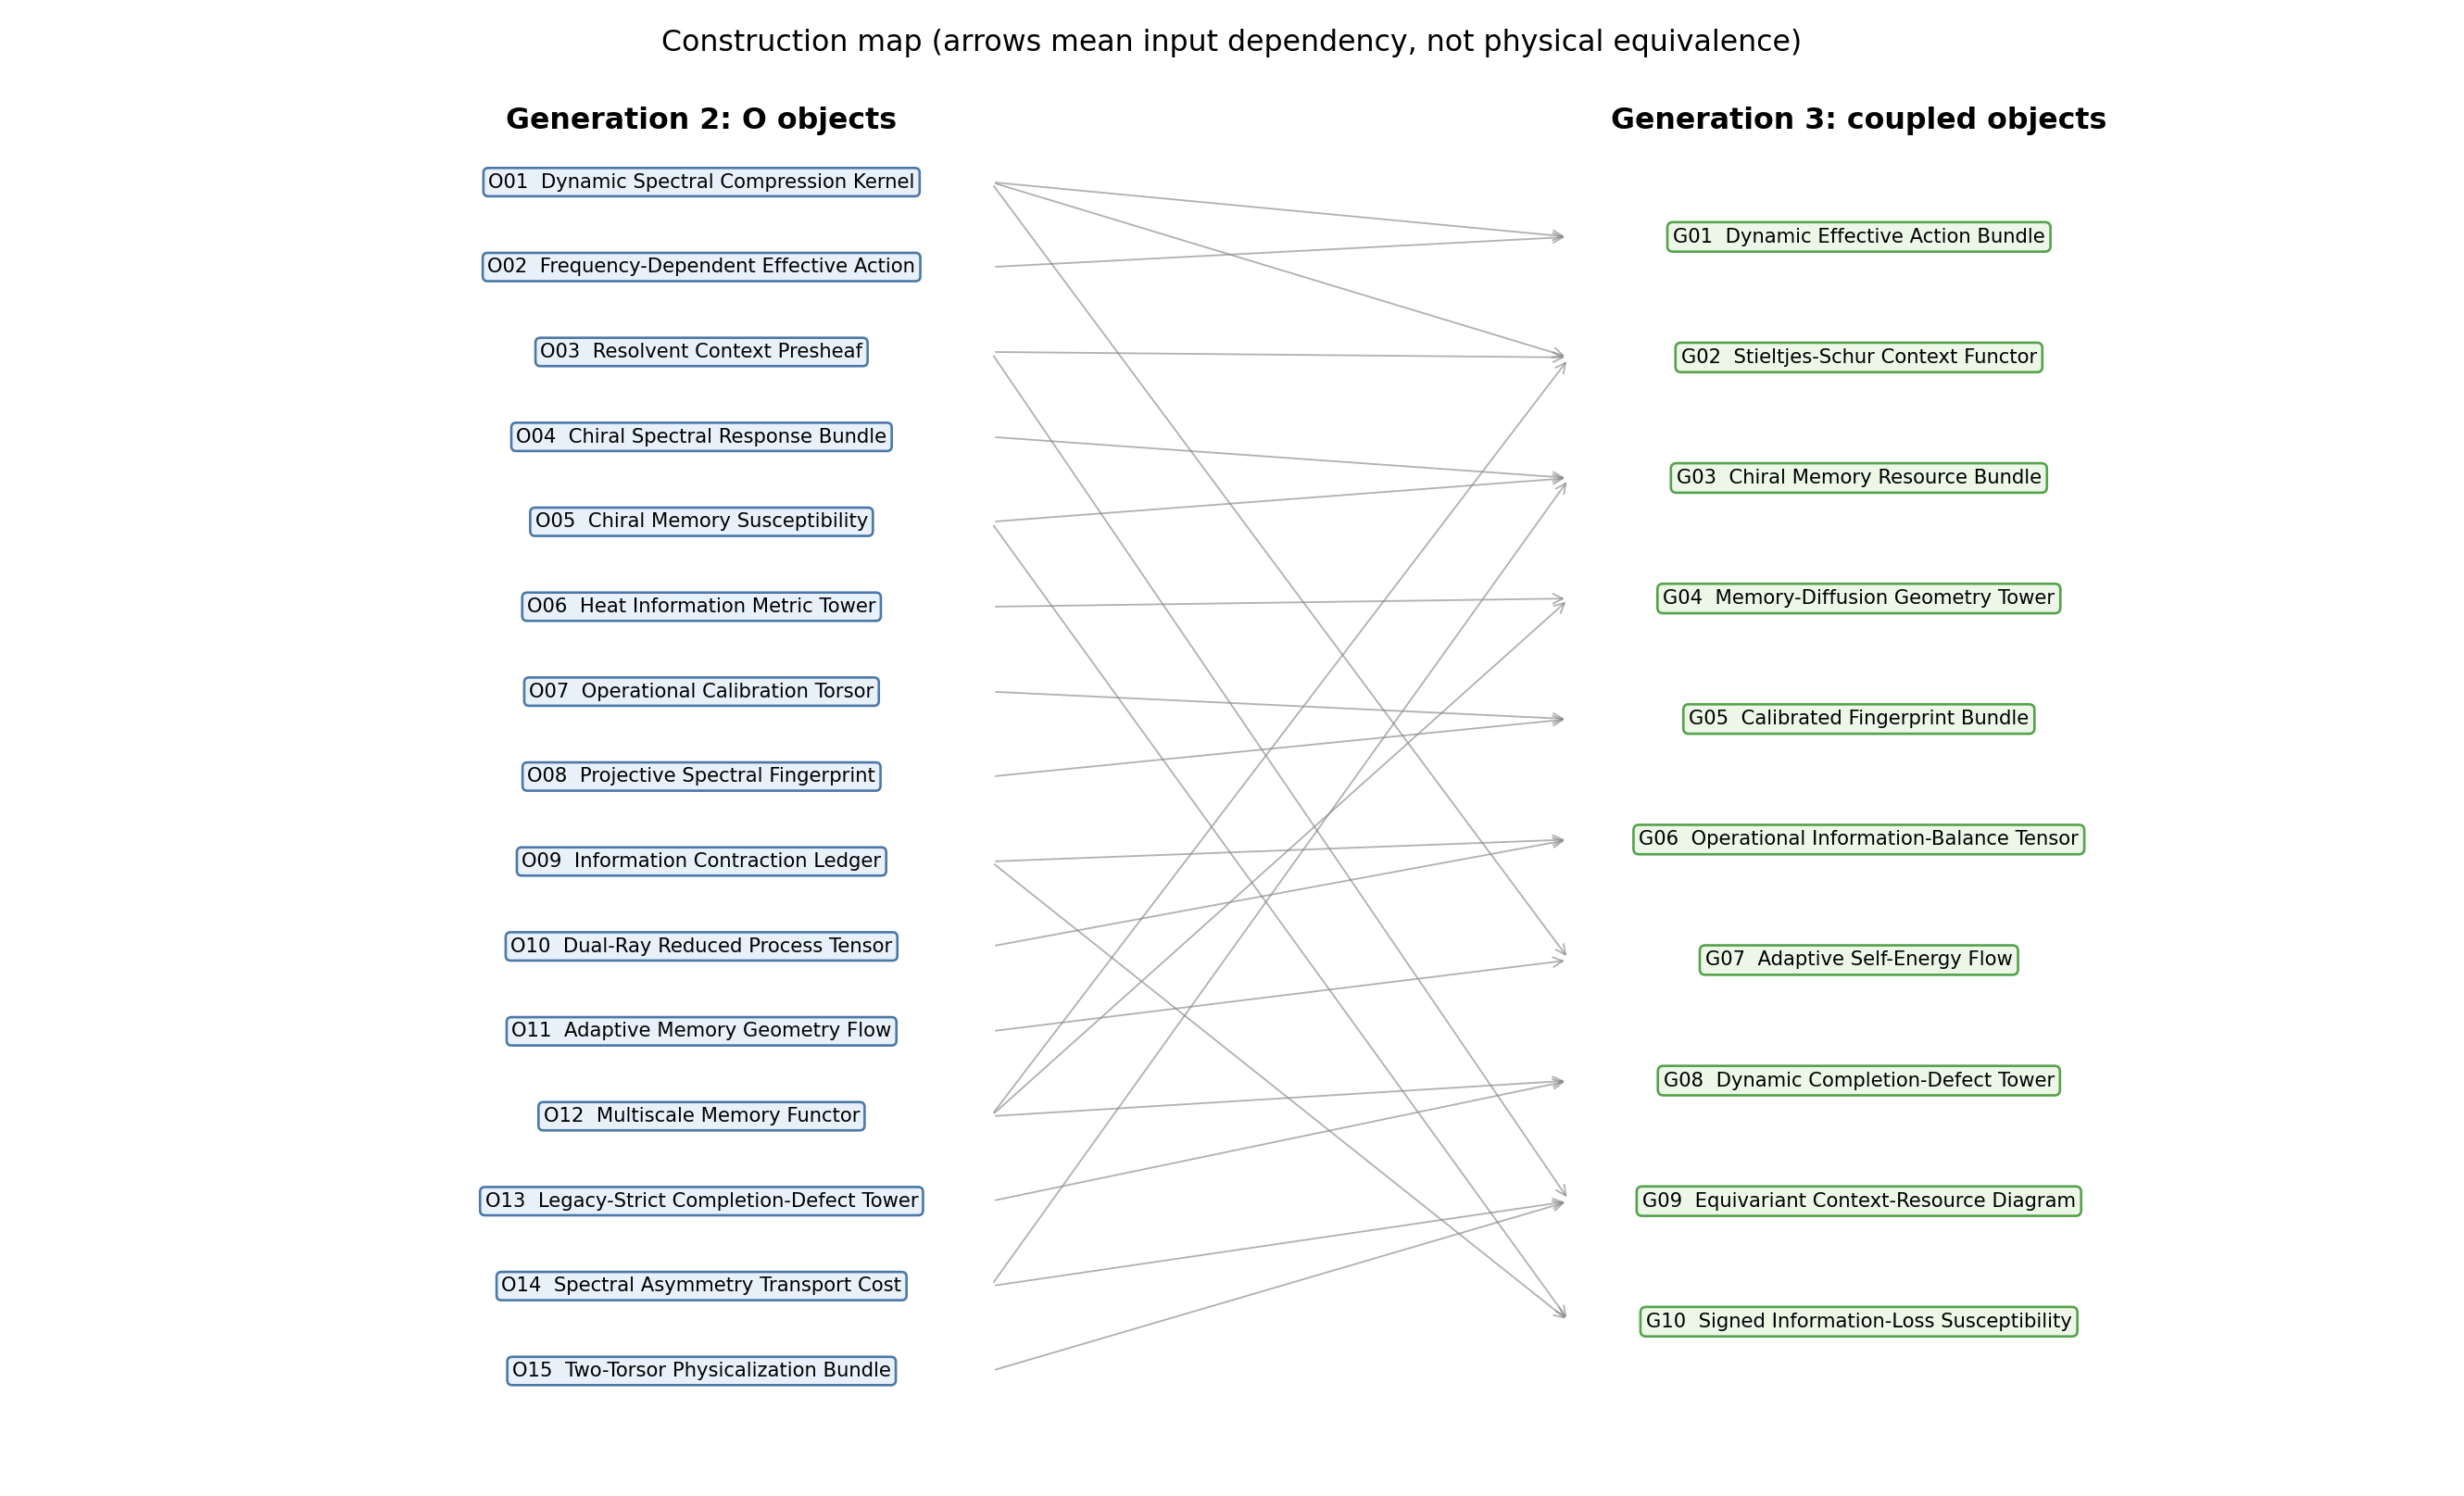
\includegraphics[width=0.97\textwidth]{FIN_Second_Generation_Atlas_Figures/generation2_generation3_map.png}
\caption{Input dependencies between the O and G generations. Arrows do not assert physical equivalence.}
\end{figure}

\begin{center}
\begingroup\fontsize{7}{8.4}\selectfont
\setlength{\tabcolsep}{2.5pt}
\renewcommand{\arraystretch}{1.16}
\begin{longtable}{@{}p{0.055\textwidth}p{0.136\textwidth}p{0.266\textwidth}p{0.328\textwidth}p{0.074\textwidth}@{}}
\toprule
\textbf{ID} & \textbf{Combination} & \textbf{Higher-order object} & \textbf{Definition/\allowbreak{}role} & \textbf{Status} \\
\midrule
\endhead
G01 & O01+O02 & Dynamic Effective Action Bundle & Stieltjes self-energy plus exact source action & \statusProven{} \\
G02 & O01+O03+O12 & Stieltjes--Schur Context Functor & contexts, compatible reductions, completely monotone self-energies & \statusProven{} \\
G03 & O04+O05+O14 & Chiral Memory Resource Bundle & odd memory susceptibility plus asymmetry-resource budget & \statusStrong{} \\
G04 & O06+O12 & Memory--Diffusion Geometry Tower & geometry indexed by diffusion time and hiding depth & \statusModerate{} \\
G05 & O07+O08 & Calibrated Fingerprint Bundle & scale-free test plus explicitly external scale section & \statusProven{} \\
G06 & O09+O10 & Operational Information-Balance Tensor & multitime information-contraction ledger & \statusModerate{} \\
G07 & O01+O11 & Adaptive Self-Energy Flow & learned trajectory in Stieltjes-function space & \statusSpeculative{} \\
G08 & O12+O13 & Dynamic Completion-Defect Tower & tests whether bridge defect survives dynamic reduction & \statusModerate{} \\
G09 & O03+O14+O15 & Equivariant Context-Resource Diagram & contexts, scale, orientation as separate sectional structures & \statusSpeculative{} \\
G10 & O05+O09 & Signed Information-Loss Susceptibility & derivative of information contraction with respect to chiral twist & \statusSpeculative{} \\
\bottomrule
\end{longtable}
\endgroup
\end{center}

\chapter{Principal "shadow shapes"}

\section{Shadow 1 --- the missing object space is Stieltjes space}

Rather than ask which next static kernel arises after compression, the Green+Schur+dynamics combination shows that the proper object is the function \(z\mapsto\Sigma(z)\). The self-similarity question changes from "is \(K\) a fixed point?" to "is the family of memory functions closed or attracted to a fixed class?" \textbf{\statusStrong{}} as a direction; no fixed point was found.

\section{Shadow 2 --- observation and compression both select context}

Compression selects retained degrees of freedom; an observer selects accessible observables. Their common shadow is the context \(E\) and its effective operator \(B_E(z)\). \textbf{\statusModerate{}} Physical observation is not thereby reduced to a Schur complement: an instrument and record remain necessary.

\section{Shadow 3 --- "negative information" is often flow into an invisible sector}

O09 and O01 suggest

\[
\text{loss of accessible distinguishability}
\longleftrightarrow
\text{correlations/excursions in sector }H.
\]

Information may remain in a full reversible description while disappearing from the selected record. \textbf{\statusStrong{}}

\section{Shadow 4 --- chirality is a tangent, not a point}

\[
\Xi_E\in T_{\Sigma_E}\operatorname{Stieltjes}_+(E).
\]

Orientation appears as a direction in memory-operator space. This new derived characteristic does not choose whether that tangent is positive or negative. \textbf{\statusStrong{}}

\section{Shadow 5 --- physicalization requires two sections and one process}

The smallest shadow of missing physics consists of three independent elements: a scale section, an orientation/\allowbreak{}sector section, and an operational process with preparation, instrument, and record. None substitutes for either of the others. \textbf{\statusProven{}} as a separation of types.

\section{Shadow 6 --- adaptation may act on memory rather than directly on a kernel}

Instead of

\[
\dot K=-\nabla_K\mathcal L,
\]

the natural object may be

\[
\partial_t\Sigma(z;t)
=-\operatorname{grad}_{\Sigma}\mathcal L_{\rm process}.
\]

\textbf{\statusSpeculative{}} Positivity and complete monotonicity could constrain the learning law.

\section{Shadow 7 --- the bridge defect may be dynamic}

Legacy and strict may differ not only by their distance profile but by hidden memory structure. O13/\allowbreak{}G08 can test whether the defect decays, remains constant, grows, or leaves the Stieltjes class. None of these outcomes is a bridge by assumption; it is a new falsifiable atom.

\chapter{Falsification of the strongest interpretations}

\section{Is G02 a new category theory?}

No. \textbf{\statusRefuted{}} Schur associativity and context diagrams are known mathematics. Potential novelty lies in using them to organize FIN.

\section{Does O05 solve the selector problem?}

No. \textbf{\statusRefuted{}} The family \(A(\theta)\) requires \(\theta\), and inversion maps \(\theta\) to \(-\theta\), producing the pair \(\pm\Xi\). O05 is a new receiver.

\section{Is O09 physical entropy?}

Not without additional data. \textbf{\statusRefuted{}} Thermodynamics requires at least a temperature, Hamiltonian, protocol, and an apparatus/\allowbreak{}reset ledger.

\section{Does O12 prove a fractal fixed point?}

No. \textbf{\statusRefuted{}} O12 defines the right search space. Existence of an attractor or self-similar operator measure remains open.

\section{Does O11 prove that FIN is biological?}

No. \textbf{\statusRefuted{}} Neural operators, reservoir computing, and plasticity provide mechanistic analogies, but no empirical map.

\section{Does G09 provide a global section?}

No on current artifacts. \textbf{\statusRefuted{}} The sectional language exposes the obstruction; it removes neither QW-2191 nor the scale orbit.

\chapter{Research programs 255--266}

\begin{enumerate}
\item 
\textbf{P255 --- Stieltjes theorem for all contexts.} Prove positivity, complete monotonicity, operator-measure representation, and the limits at zero and infinity. Probability: 0.95.

\item 
\textbf{P256 --- Minimal realization of self-energy.} Classify hidden pairs \((A_{HH},A_{HE})\) producing the same \(\Sigma_E(z)\). Probability: 0.85.

\item 
\textbf{P257 --- Formalize the context functor.} Define the category and verify Schur associativity in a proof assistant or independent algebraic core. Probability: 0.80.

\item 
\textbf{P258 --- Analytic chiral memory susceptibility.} Derive \(\Xi_E(z)\), covariance, and norm bounds while separating gauge convention from flux observable. Probability: 0.82.

\item 
\textbf{P259 --- Dynamic RG in Stieltjes space.} Define \(\mathcal R:\Sigma^{(n)}\mapsto\Sigma^{(n+1)}\) and search for fixed points, cycles, or no-go results. Probability: 0.45; high reward.

\item 
\textbf{P260 --- Multitime information-balance tensor.} Extend O09 to a process ledger separating system, apparatus, and hidden-node contraction. Probability: 0.75.

\item 
\textbf{P261 --- Dynamic completion-defect test.} Freeze one map and test \(\Delta_\Sigma(z)=\Sigma_{\rm strict}(z)-
   \mathcal C_\Sigma[\Sigma_{\rm legacy}(z)]\), without fitting after seeing the target. Bridge probability: 0.30; valuable no-go: 0.80.

\item 
\textbf{P262 --- Calibrated Fingerprint Experiment.} Test spectral ratios first, then independently calibrate \(\tau\), with no post-unblinding changes. Methodological success: 0.75.

\item 
\textbf{P263 --- Tomography of currents and chiral memory.} Measure \(C_d\), \(d=1,\ldots,5\), and intermediate interventions; test \(C_\chi\) and \(\Xi_E(z)\) separately. Probability: 0.70.

\item 
\textbf{P264 --- False-positive atlas O01--O10.} Quantify how often random and structured Laplacians pass the FIN tests. Probability: 0.90.

\item 
\textbf{P265 --- Identifiability of Adaptive Memory Geometry.} Compare genuine generator drift with static operators, apparatus memory, and calibration errors using hold-out data. Probability: 0.65.

\item 
\textbf{P266 --- Biological/\allowbreak{}cybernetic benchmark.} Test fading-memory capacity, robustness--plasticity, recovery, and readout dimension against matched standard reservoirs. Probability: 0.72.

\end{enumerate}

\chapter{Strategic priority}

\begin{center}
\begingroup\small
\setlength{\tabcolsep}{2.5pt}
\renewcommand{\arraystretch}{1.16}
\begin{longtable}{@{}p{0.160\textwidth}p{0.280\textwidth}p{0.420\textwidth}@{}}
\toprule
\textbf{Rank} & \textbf{Program} & \textbf{Reason} \\
\midrule
\endhead
1 & P255 & near-certain formal closure of the new object space \\
2 & P256 & determines what can be inferred about the hidden sector \\
3 & P258 & closes the new chiral-memory characteristic without selector claim \\
4 & P257 & protects context language against metaphorical use \\
5 & P264 & measures specificity of the atlas \\
6 & P260 & joins information to a complete process \\
7 & P262 & moves the result toward the laboratory \\
8 & P263 & separates harmonics from memory experimentally \\
9 & P259 & highest mathematical reward, high risk \\
10 & P261 & one honest bridge attack \\
11 & P265 & tests adaptation and identifiability \\
12 & P266 & controls biological/\allowbreak{}cybernetic analogies \\
\bottomrule
\end{longtable}
\endgroup
\end{center}

\chapter{Guardrail-compatible boundaries}

This report does not export a non-premise strict selector, discharge QW-2191, a canonical unit of length/\allowbreak{}time/\allowbreak{}mass/\allowbreak{}energy/\allowbreak{}action, a complete legacy-to-strict map, role transfer for \(\sin^2\theta_W\), \(\alpha_{\rm EM}\), or the gravity hierarchy, a strict-source adaptive law, \(L_{\rm total}\), the Standard Model, GR, a ToE, a physical observer, environment or apparatus, or external data validation.

The nadsoliton remains primordial information in a solitonic state. The contexts \(E/H\) partition accessibility of its degrees of freedom; they are not a separate informational layer beneath it.

\chapter{Final verdict}

The most important derived structure is neither another kernel nor another constant. It is

\[
\boxed{\text{the Stieltjes--Schur Context Functor}},
\]

a contextual family of exact effective operators whose self-energies are completely monotone, whose reductions compose, and whose time transforms generate memory.

It organizes the common shadow

\[
\text{Green}\leftrightarrow\text{compression}
\leftrightarrow\text{memory}\leftrightarrow\text{observer}
\leftrightarrow\text{accessible information}.
\]

The most interesting new tangent characteristic is \(\Xi_E(z)\), the chiral memory susceptibility. The most defensible account of information loss is \(\mathcal L_t\), contraction of accessible distinguishability. The central no-go remains the absence of orientation and scale sections.

This does not establish FIN as physics. It does provide a rigorous new object space in which subsequent questions are better typed and easier to falsify.

\chapter{Comparative literature}

\begin{enumerate}
\item 
Dörfler, F.; Bullo, F., \emph{Kron Reduction of Graphs with Applications to Electrical Networks}, \href{https://arxiv.org/abs/1102.2950}{https:/\allowbreak{}/\allowbreak{}arxiv.org/\allowbreak{}abs/\allowbreak{}1102.2950}.

\item 
Lin, Y. T.; Tian, Y.; Anghel, M.; Livescu, D., \emph{Data-driven learning for the Mori--Zwanzig formalism}, \href{https://arxiv.org/abs/2101.05873}{https:/\allowbreak{}/\allowbreak{}arxiv.org/\allowbreak{}abs/\allowbreak{}2101.05873}.

\item 
Pollock, F. A. et al., \emph{Non-Markovian quantum processes: complete framework and efficient characterisation}, \href{https://arxiv.org/abs/1512.00589}{https:/\allowbreak{}/\allowbreak{}arxiv.org/\allowbreak{}abs/\allowbreak{}1512.00589}.

\item 
Marvian, I.; Spekkens, R. W., \emph{Modes of asymmetry}, \href{https://arxiv.org/abs/1312.0680}{https:/\allowbreak{}/\allowbreak{}arxiv.org/\allowbreak{}abs/\allowbreak{}1312.0680}.

\item 
Coifman, R. R.; Lafon, S., \emph{Diffusion maps}, \href{https://doi.org/10.1016/j.acha.2006.04.006}{https:/\allowbreak{}/\allowbreak{}doi.org/\allowbreak{}10.1016/\allowbreak{}j.acha.2006.04.006}.

\item 
Shuman, D. I. et al., \emph{The Emerging Field of Signal Processing on Graphs}, \href{https://arxiv.org/abs/1211.0053}{https:/\allowbreak{}/\allowbreak{}arxiv.org/\allowbreak{}abs/\allowbreak{}1211.0053}.

\item 
Kovachki, N. et al., \emph{Neural Operator: Learning Maps Between Function Spaces}, \href{https://arxiv.org/abs/2108.08481}{https:/\allowbreak{}/\allowbreak{}arxiv.org/\allowbreak{}abs/\allowbreak{}2108.08481}.

\item 
Abramsky, S.; Brandenburger, A., \emph{The Sheaf-Theoretic Structure of Non-Locality and Contextuality}, \href{https://arxiv.org/abs/1102.0264}{https:/\allowbreak{}/\allowbreak{}arxiv.org/\allowbreak{}abs/\allowbreak{}1102.0264}.

\item 
Chamseddine, A. H.; Connes, A., \emph{The Spectral Action Principle}, \href{https://arxiv.org/abs/hep-th/9606001}{https:/\allowbreak{}/\allowbreak{}arxiv.org/\allowbreak{}abs/\allowbreak{}hep-th/\allowbreak{}9606001}.

\end{enumerate}

\chapter{Reproducible artifacts}

\begin{itemize}
\item 
fin\_nadsoliton\_second\_generation\_atlas.py

\item 
FIN\_Second\_Generation\_Combination\_Search.csv

\item 
FIN\_Second\_Generation\_Derived\_Objects.csv

\item 
FIN\_Second\_Generation\_Generation3.csv

\item 
FIN\_Second\_Generation\_Atlas\_Results.json

\item 
FIN\_Second\_Generation\_Atlas\_Figures/\allowbreak{}combination\_search\_coverage.png

\item 
FIN\_Second\_Generation\_Atlas\_Figures/\allowbreak{}derived\_object\_score\_matrix.png

\item 
FIN\_Second\_Generation\_Atlas\_Figures/\allowbreak{}generation2\_generation3\_map.png

\item 
FIN\_Second\_Generation\_Atlas\_Derived\_Nadsoliton\_Objects\_EN.md

\end{itemize}


\clearpage
\chapter*{Reproduction certificate}
\addcontentsline{toc}{chapter}{Reproduction certificate}
\begin{Verbatim}[fontsize=\small]
MPLCONFIGDIR=/tmp/matplotlib-second \
python3 fin_nadsoliton_second_generation_atlas.py
\end{Verbatim}
Expected coverage: 305 combinations, 15 O-generation objects, and 10
G-generation objects. The construction grammar is a candidate filter, not
proof of equivalence or physical realization.
\end{document}
